\documentclass[10pt]{article}
\usepackage{amsmath, amssymb, tikz-cd, array}
\usetikzlibrary{shapes.geometric}

\begin{document}

\begin{center}
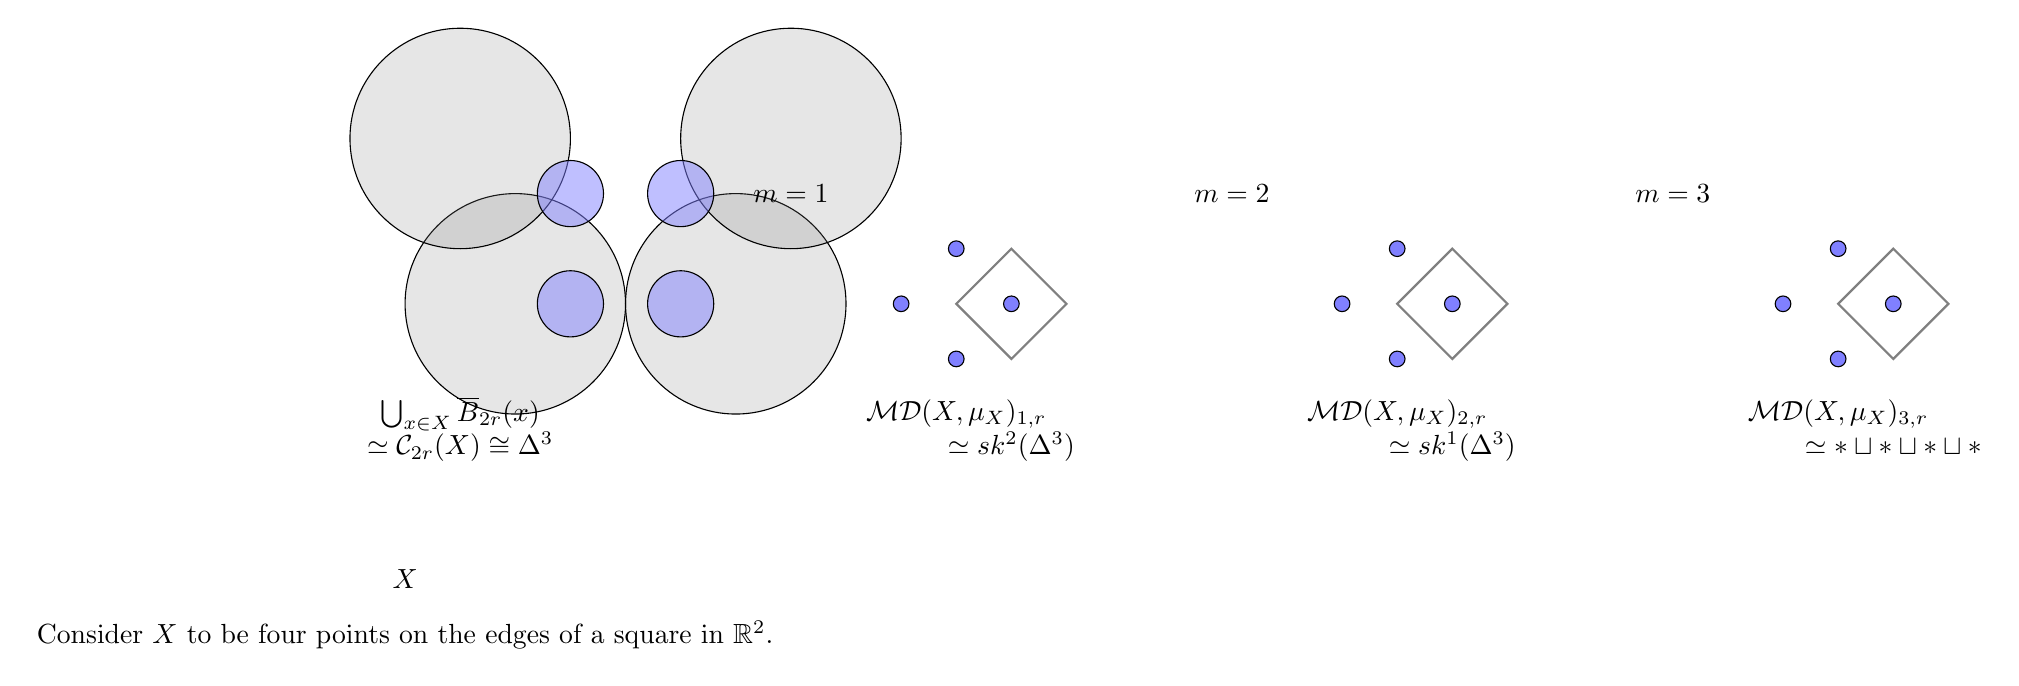
\begin{tikzpicture}[scale=0.7]
  \draw[fill=gray, fill opacity=0.2] (0,0) circle (2);
  \draw[fill=gray, fill opacity=0.2] (4,0) circle (2);
  \draw[fill=gray, fill opacity=0.2] (-1,3) circle (2);
  \draw[fill=gray, fill opacity=0.2] (5,3) circle (2);

  \draw[fill=blue!50, fill opacity=0.5] (1,2) circle (0.6);
  \draw[fill=blue!50, fill opacity=0.5] (3,2) circle (0.6);
  \draw[fill=blue!50, fill opacity=0.5] (1,0) circle (0.6);
  \draw[fill=blue!50, fill opacity=0.5] (3,0) circle (0.6);

  \node at (-1,-2) {$\bigcup_{x\in X}\overline{B}_{2r}(x)$};
  \node at (-1,-2.6) {$\simeq\mathcal{C}_{2r}(X)\cong\Delta^3$};

  \begin{scope}[shift={(8,0)}]
    \foreach \i in {1,...,4} {
      \node[circle, draw, fill=blue!50, scale=0.6] at ({90*(\i-1)}:1) {};
    }
    \draw[thick, gray] (0,0) -- (1,1) -- (2,0) -- (1,-1) -- cycle;
  \end{scope}

  \begin{scope}[shift={(16,0)}]
    \foreach \i in {1,...,4} {
      \node[circle, draw, fill=blue!50, scale=0.6] at ({90*(\i-1)}:1) {};
    }
    \draw[thick, gray] (0,0) -- (1,1) -- (2,0) -- (1,-1) -- cycle;
  \end{scope}

  \begin{scope}[shift={(24,0)}]
    \foreach \i in {1,...,4} {
      \node[circle, draw, fill=blue!50, scale=0.6] at ({90*(\i-1)}:1) {};
    }
    \draw[thick, gray] (0,0) -- (1,1) -- (2,0) -- (1,-1) -- cycle;
  \end{scope}

  \node at (5,2) {$m=1$};
  \node at (13,2) {$m=2$};
  \node at (21,2) {$m=3$};

  \node at (8,-2) {$\mathcal{MD}(X,\mu_X)_{1,r}$};
  \node at (9,-2.6) {$\simeq sk^2(\Delta^3)$};

  \node at (16,-2) {$\mathcal{MD}(X,\mu_X)_{2,r}$};
  \node at (17,-2.6) {$\simeq sk^1(\Delta^3)$};

  \node at (24,-2) {$\mathcal{MD}(X,\mu_X)_{3,r}$};
  \node at (25,-2.6) {$\simeq\ast\sqcup\ast\sqcup\ast\sqcup\ast$};
  
  \node at (-2,-5) {$X$};
  \node at (-2,-6) {$\text{Consider } X \text{ to be four points on the edges of a square in } \mathbb{R}^2.$};

\end{tikzpicture}
\end{center}

\end{document}